\section{Video and I/O devices}
\label{sec:videoio}

\subsection{Video}

The video block is in \src{rtl/video.vhd}. The output is the VGA mode 640 $\times$ 400 at 70 Hz. This is the mode that Doom used on a PC. The framebuffer is 320 $\times$ 200 pixels. The video block shows each framebuffer pixel as a 2 $\times$ 2 block, and the picture uses all 400 lines (Figure~\ref{fig:screen}).

The monitor shows the 400 lines on the full height of its 4:3 screen. Thus each framebuffer pixel is 1.2 times as high as it is wide. The Doom graphics were drawn for this pixel shape.

\begin{figure}[H]
  \centering
  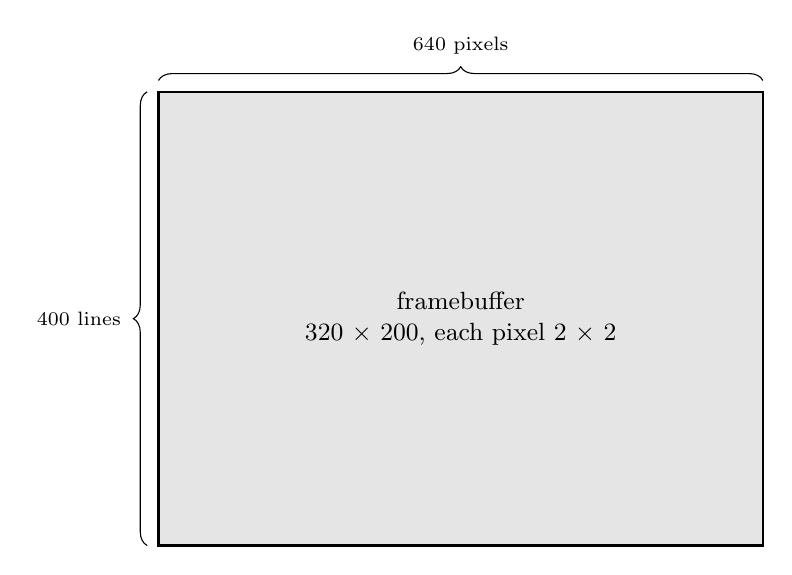
\begin{tikzpicture}[x=0.012cm, y=0.0144cm, font=\scriptsize]
    \fill[black!10] (0,0) rectangle (640,400);
    \draw[thick] (0,0) rectangle (640,400);
    \node[align=center, font=\small] at (320,200) {framebuffer\\320 $\times$ 200, each pixel 2 $\times$ 2};
    \draw[decorate, decoration={brace, amplitude=5pt}] (0,410) -- (640,410) node[midway, above=6pt] {640 pixels};
    \draw[decorate, decoration={brace, amplitude=5pt}] (-12,0) -- (-12,400) node[midway, left=6pt] {400 lines};
  \end{tikzpicture}
  \caption{The screen layout, as a 4:3 monitor shows it}
  \label{fig:screen}
\end{figure}

\subsubsection{Timing}
The pixel rate is 25 MHz. The signal \texttt{pix\_en} is high in each second clock cycle, and the counters change only when \texttt{pix\_en} is high. The horizontal counter \texttt{h} counts 0 to 799. The vertical counter \texttt{v} counts 0 to 448. Table~\ref{tab:vga} and Figure~\ref{fig:vgatiming} give the timing.

The horizontal sync is active low and the vertical sync is active high. A monitor uses these polarities to identify the 400-line mode. The 640 $\times$ 480 mode has the same horizontal timing, but its two sync signals are active low.

\begin{guidetable}{VGA timing}{vga}{l c c c c c}
 & visible & front porch & sync & back porch & total \\
\midrule
horizontal (pixels) & 640 & 16 & 96 & 48 & 800 \\
counter \texttt{h} & 0 to 639 & 640 to 655 & 656 to 751 & 752 to 799 & \\
\midrule
vertical (lines) & 400 & 12 & 2 & 35 & 449 \\
counter \texttt{v} & 0 to 399 & 400 to 411 & 412 to 413 & 414 to 448 & \\
\end{guidetable}

\begin{figure}[H]
  \centering
  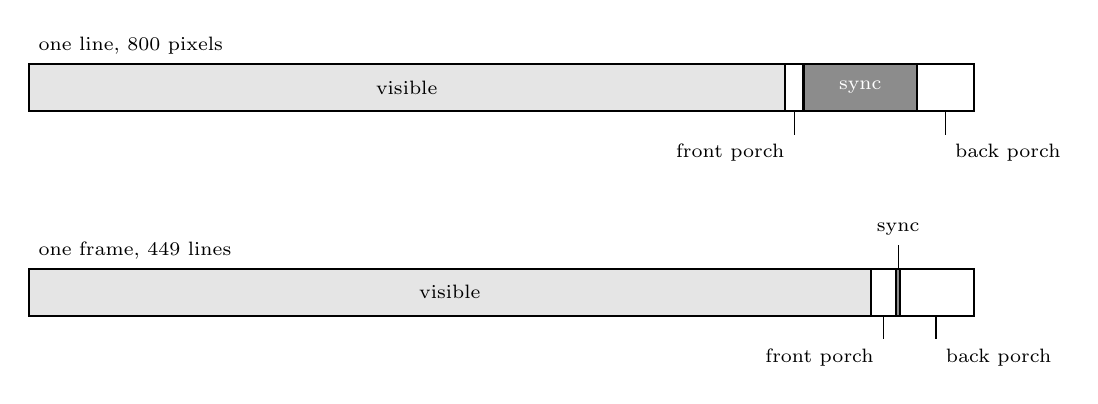
\begin{tikzpicture}[x=0.015cm, y=1cm, font=\scriptsize]
    \node[above right] at (0,0.6) {one line, 800 pixels};
    \draw[thick, fill=black!10] (0,0) rectangle (640,0.6);   \node at (320,0.3) {visible};
    \draw[thick, fill=white]    (640,0) rectangle (656,0.6);
    \draw[thick, fill=black!45] (656,0) rectangle (752,0.6); \node[white] at (704,0.3) {sync};
    \draw[thick, fill=white]    (752,0) rectangle (800,0.6);
    \draw (648,0) -- (648,-0.3) node[below left] {front porch};
    \draw (776,0) -- (776,-0.3) node[below right] {back porch};
    \begin{scope}[yshift=-2.6cm, x=0.026726cm]
      \node[above right] at (0,0.6) {one frame, 449 lines};
      \draw[thick, fill=black!10] (0,0) rectangle (400,0.6);   \node at (200,0.3) {visible};
      \draw[thick, fill=white]    (400,0) rectangle (412,0.6);
      \draw[thick, fill=black!45] (412,0) rectangle (414,0.6);
      \draw[thick, fill=white]    (414,0) rectangle (449,0.6);
      \draw (406,0) -- (406,-0.3) node[below left] {front porch};
      \draw (413,0.6) -- (413,0.9) node[above] {sync};
      \draw (431,0) -- (431,-0.3) node[below right] {back porch};
    \end{scope}
  \end{tikzpicture}
  \caption{VGA timing, to scale}
  \label{fig:vgatiming}
\end{figure}

One frame is $800 \times 449$ pixels at two clock cycles for each pixel, which is 718,400 cycles. The frame rate is 69.6 Hz.

\subsubsection{Datapath}
Figure~\ref{fig:video} shows the datapath. It has these parts:

\begin{itemize}
  \item The line fetcher reads one framebuffer line from SRAM through the video port.
  \item The line buffer is an M4K RAM of 1024 halfwords. It holds two lines.
  \item In 8-bit mode, each byte from the line buffer is a palette index. The palette is an M4K RAM of 256 entries of 12 bits.
  \item In RGB565 mode, each halfword from the line buffer is one pixel, and the palette is not used.
  \item The DAC on the DE1 has 4 bits for each of red, green and blue.
\end{itemize}

\begin{figure}[H]
  \centering
  \begin{tikzpicture}[font=\scriptsize]
    \node[ram, minimum width=1.8cm, minimum height=1.4cm] (sram) at (0,0) {SRAM\\controller};
    \node[blk, minimum width=1.8cm, minimum height=1.2cm] (fetch) at (0,2.8) {line\\fetcher};
    \node[ram, minimum width=2.0cm, minimum height=1.4cm] (lb) at (3.6,0) {line buffer\\1024 $\times$ 16};
    \node[mux, minimum height=1.2cm, minimum width=0.5cm] (bs) at (6.6,0) {};
    \node[ram, minimum width=1.8cm, minimum height=1.4cm] (pal) at (8.9,0) {palette\\256 $\times$ 12};
    \node[mux, minimum height=1.6cm, minimum width=0.55cm] (md) at (11.3,-0.4) {};
    \node[blk, minimum width=1.4cm, minimum height=1.4cm] (dac) at (13.2,-0.4) {VGA\\DAC};
    \draw[sig] (-0.4,2.2) -- (-0.4,0.7);
    \draw[sig] (0.4,0.7) -- (0.4,2.2);
    \node[left] at (-0.4,1.45) {\texttt{v\_req}, \texttt{v\_addr}};
    \node[right] at (0.4,1.45) {\texttt{v\_ack}};
    \draw[sig] (sram.east) -- (lb.west);
    \node[above] at (1.75,0) {\texttt{v\_data}};
    \draw[sig] (fetch.east) -| (lb.north);
    \node[above] at (2.3,2.8) {write address};
    \draw[sig] (4.6,0.3) -- (6.35,0.3);
    \draw[sig] (4.6,-0.3) -- (6.35,-0.3);
    \node[above] at (5.45,0.3) {low byte};
    \node[below] at (5.45,-0.3) {high byte};
    \draw[thick] (6.6,0.6) -- (6.6,1.0) node[above] {\texttt{h[1]}};
    \draw[sig] (bs.east) -- (pal.west);
    \node[above] at (7.4,0) {index};
    \draw[sig] (pal.east) -- (11.02,0);
    \draw[sig] (3.6,-0.7) -- (3.6,-1.7) -- (10.4,-1.7) -- (10.4,-0.8) -- (11.02,-0.8);
    \node[below] at (7.0,-1.7) {RGB565 pixel};
    \draw[thick] (11.3,0.4) -- (11.3,1.0) node[above] {VIDEO\_MODE};
    \draw[sig] (md.east) -- (dac.west);
    \node[above] at (12.05,-0.4) {12};
  \end{tikzpicture}
  \caption{The video datapath}
  \label{fig:video}
\end{figure}

The read path has three register stages: the line buffer, the palette and the output register. The video block delays the sync signals and the blanking signal by three cycles, so they align with the pixel data.

\subsubsection{Line fetch}
Each framebuffer row is on the screen for two VGA lines. The screen shows row $k$ on VGA lines $2k$ and $2k + 1$. The line fetcher reads row $k$ during the line before, which is VGA line $2k - 1$. For row 0, this is line 448, the last line of the frame (Figure~\ref{fig:linefetch}).

The line buffer has two halves. The line fetcher writes one half while the screen shows the other half. Even rows use half 0 and odd rows use half 1.

\begin{figure}[H]
  \centering
  \begin{waveform}[1.4cm]{8}
    \wavebus{VGA line}{0/1/447, 1/2/448, 2/3/0, 3/4/1, 4/5/2, 5/6/3, 6/7/4, 7/8/5}
    \wavebus{on screen}{0/2/blanking, 2/4/row 0, 4/6/row 1, 6/8/row 2}
    \wavebus{fetch}{0/1/x, 1/2/row 0, 2/3/x, 3/4/row 1, 4/5/x, 5/6/row 2, 6/7/x, 7/8/row 3}
    \wavebus{write half}{0/1/x, 1/2/0, 2/3/x, 3/4/1, 4/5/x, 5/6/0, 6/7/x, 7/8/1}
    \wavebus{read half}{0/2/x, 2/4/0, 4/6/1, 6/8/0}
  \end{waveform}
  \caption{The line fetch sequence at the start of a frame}
  \label{fig:linefetch}
\end{figure}

A line fetch is 160 halfword reads in 8-bit mode and 320 in RGB565 mode. Each read takes three cycles (Section~\ref{sec:memory}). Thus a line fetch takes approximately 480 or 960 cycles. One VGA line is 1600 cycles.

\subsubsection{Framebuffer address}
Software writes the framebuffer address to \texttt{FB\_BASE}. The video block does not use the new value immediately. It copies \texttt{FB\_BASE} and \texttt{VIDEO\_MODE} at the start of vertical blanking, when line 399 ends. \texttt{FRAME\_COUNT} increments in the same cycle.

Thus the picture always comes from one complete framebuffer. Software reads \texttt{FRAME\_COUNT} to find when the video block has changed to the new framebuffer.

\subsubsection{Pixel formats}
Figure~\ref{fig:palreg} shows the \texttt{PALETTE} register and an RGB565 pixel. The hardware uses the top 4 bits of each color.

\begin{figure}[H]
  \centering
  \begin{bitfield}[scale=0.88]{32}
    \bitname{PALETTE}
    \bits{31}{24}{index}\bits{23}{20}{R}\bits*{19}{16}{}\bits{15}{12}{G}\bits*{11}{8}{}\bits{7}{4}{B}\bits*{3}{0}{}
  \end{bitfield}

  \medskip
  \begin{bitfield}[scale=0.88]{16}
    \bitname{RGB565}
    \bits{15}{12}{R}\bits*{11}{11}{}\bits{10}{7}{G}\bits*{6}{5}{}\bits{4}{1}{B}\bits*{0}{0}{}
  \end{bitfield}
  \caption{The color formats. The hardware ignores the gray bits.}
  \label{fig:palreg}
\end{figure}

\subsection{I/O registers}

The I/O block is in \src{rtl/io.vhd}. The registers in Table~\ref{tab:ioregs} are at \texttt{0xF000\_0000}. All registers are 32 bits, and software must use word access.

\begin{guidetable}{I/O registers at \texttt{0xF000\_0000}}{ioregs}{l l c p{0.55\linewidth}}
offset & name & access & function \\
\midrule
\texttt{0x00} & UART\_DATA & W & Send byte [7:0]. Write only when \texttt{tx\_ready} is 1. \\
\texttt{0x00} & UART\_DATA & R & Bit 31 = byte valid, [7:0] = received byte. A read removes the byte. \\
\texttt{0x04} & UART\_STATUS & R & Bit 0 = \texttt{tx\_ready}. \\
\texttt{0x08} & TIMER\_US & R & Microseconds since configuration. \\
\texttt{0x0C} & TIMER\_CYCLES & R & Clock cycles since configuration. \\
\texttt{0x10} & KBD & R & Bit 8 = valid, [7:0] = PS/2 byte. A read removes the byte from the FIFO. \\
\texttt{0x14} & SWITCHES & R & [9:0] = SW, [19:16] = KEY (1 = not pushed). \\
\texttt{0x18} & LEDR & W & [8:0]. LEDR9 shows the \texttt{halted} output of the CPU. \\
\texttt{0x1C} & LEDG & W & [7:0]. \\
\texttt{0x20} & HEX & W & [15:0], shown as four hex digits on HEX3 to HEX0. \\
\texttt{0x30} & FB\_BASE & RW & Byte offset of the framebuffer in SRAM. \\
\texttt{0x34} & FRAME\_COUNT & R & Number of vertical blanking periods. \\
\texttt{0x38} & PALETTE & W & See Figure~\ref{fig:palreg}. \\
\texttt{0x3C} & VIDEO\_MODE & RW & Bit 0 = RGB565 mode. \\
\texttt{0x40} & JTAG\_DATA & R & Next word from the JTAG loader. A read removes the word. \\
\texttt{0x44} & JTAG\_STATUS & R & Bit 0 = word available. Bit 1 = FIFO overflow. \\
\end{guidetable}

A KEY0 reset does not clear the timers, \texttt{FRAME\_COUNT}, the LEDs, \texttt{HEX} or \texttt{FB\_BASE}. Only FPGA configuration sets their initial values.

The keyboard FIFO holds 16 bytes. If the FIFO is full, the I/O block discards a new byte.

\subsection{Interrupt controllers}

Linux uses two standard RISC-V interrupt controllers, the CLINT and the PLIC. The I/O block has a small version of each (Figure~\ref{fig:irq}, Table~\ref{tab:clint}).

\begin{itemize}
  \item The CLINT supplies the timer interrupt (MTIP) and the software interrupt (MSIP). The timer \texttt{mtime} is a 64-bit microsecond counter. \texttt{TIMER\_US} is its low word.
  \item The PLIC supplies the external interrupt (MEIP). It has one source, the PS/2 keyboard.
\end{itemize}

The 16550 console and the JTAG loader do not cause interrupts. Software polls them.

\begin{figure}[H]
  \centering
  \begin{tikzpicture}[font=\scriptsize]
    \node[ram, minimum width=1.8cm] (fifo) at (0,0) {keyboard\\FIFO};
    \node[and port, number inputs=2] (lvl) at (3.6,0) {};
    \node[blk, minimum width=3.4cm, minimum height=1.3cm] (plic) at (7.6,0) {PLIC: pending, enable,\\priority $>$ threshold};
    \draw[thick] (fifo.east) -- (1.4,0) |- (lvl.in 1);
    \node[above] at (1.9,0.28) {not empty};
    \draw[thick] (1.4,-1.0) -- (2.2,-1.0) |- (lvl.in 2);
    \node[left] at (1.4,-1.0) {RE bit of the PS/2 control register};
    \draw[sig] (lvl.out) -- (plic.west);

    \node[blk, minimum width=1.9cm] (us) at (3.2,-2.6) {\texttt{mtime}};
    \node[blk, minimum width=3.4cm] (cmp) at (7.6,-2.6) {$\mathtt{mtime} \ge \mathtt{mtimecmp}$};
    \draw[sig] (us) -- (cmp);
    \node[blk, minimum width=3.4cm] (msip) at (7.6,-4.2) {\texttt{msip} bit 0};

    \node[blk, minimum width=1.3cm, minimum height=5.4cm] (cpu) at (12.0,-2.1) {CPU\\\texttt{mip}};
    \draw[sig] (plic.east) -- (plic.east -| cpu.west);
    \draw[sig] (cmp.east) -- (cmp.east -| cpu.west);
    \draw[sig] (msip.east) -- (msip.east -| cpu.west);
    \node[above] at (10.3,0) {MEIP};
    \node[above] at (10.3,-2.6) {MTIP};
    \node[above] at (10.3,-4.2) {MSIP};
  \end{tikzpicture}
  \caption{The interrupt sources}
  \label{fig:irq}
\end{figure}

\begin{guidetable}{CLINT and PLIC registers}{clint}{l l l}
address & register & function \\
\midrule
\texttt{0xF100\_0000} & msip & Bit 0 sets MSIP. \\
\texttt{0xF100\_4000}, \texttt{+4} & mtimecmp (low, high) & Reset value is all ones. \\
\texttt{0xF100\_BFF8}, \texttt{+4} & mtime (low, high) & Read only. \\
\midrule
\texttt{0xF400\_0004} & priority of source 1 & 3 bits. \\
\texttt{0xF400\_1000} & pending & Bit 1, read only. \\
\texttt{0xF400\_2000} & enable & Bit 1. \\
\texttt{0xF420\_0000} & threshold & 3 bits. \\
\texttt{0xF420\_0004} & claim / complete & A read gives 1 and claims the interrupt. A write of 1 completes it. \\
\end{guidetable}

\subsection{System controller}

The system controller (syscon) is one write-only register at \texttt{0xF000\_2000}.

\begin{itemize}
  \item A write of \texttt{0x5555} is a power-off request. The CPU stops and HEX shows \texttt{00FF}.
  \item A write of \texttt{0x7777} resets the board. The effect is the same as a power-on reset.
\end{itemize}

\subsection{UART}

The UART is in \src{rtl/uart.vhd}. The format is 115200 baud, 8 data bits, no parity, 1 stop bit. One bit is 434 clock cycles. Figure~\ref{fig:uart} shows the frame for the byte \texttt{0x41}. The least significant bit goes first.

\begin{figure}[H]
  \centering
  \begin{waveform}[0.95cm]{12}
    \wave{\texttt{TXD}}{101000001011}
    \wavebus{bit}{0/1/idle, 1/2/start, 2/3/D0, 3/4/D1, 4/5/D2, 5/6/D3, 6/7/D4, 7/8/D5, 8/9/D6, 9/10/D7, 10/11/stop, 11/12/idle}
  \end{waveform}
  \caption{The UART frame for the byte \texttt{0x41}}
  \label{fig:uart}
\end{figure}

The receiver operates as follows:

\begin{enumerate}
  \item Wait for RXD to go low (the start bit).
  \item Wait 651 cycles (1.5 bit times). This is the middle of D0.
  \item Sample 8 data bits, one each 434 cycles.
  \item Sample the stop bit. If it is high, supply the byte. If it is low, discard the byte.
\end{enumerate}

The I/O block holds one received byte. A new byte replaces a byte that software has not read.

\subsubsection{16550 console}
The Linux serial driver needs a 16550 UART. The I/O block has a second set of registers at \texttt{0xF000\_1000} that looks like a 16550, with the registers 4 bytes apart. Only the functions that a polled driver uses are implemented: the data register, the line status bits DR and THRE, and the interrupt identification register. The divisor registers hold their value but do not change the baud rate.

A byte written to the 16550 goes to the RS-232 pin and to the JTAG console. A read takes a byte from the JTAG console first, and then from the RS-232 receiver.

\subsection{PS/2 keyboard}

The receiver is in \src{rtl/ps2_rx.vhd}. The keyboard supplies the clock and sends 11 bits for each byte (Figure~\ref{fig:ps2}).

\begin{figure}[H]
  \centering
  \begin{waveform}[0.6cm]{23}
    \wave{\texttt{PS2\_CLK}}{11010101010101010101011}
    \wavebus{\texttt{PS2\_DAT}}{1/3/0, 3/5/D0, 5/7/D1, 7/9/D2, 9/11/D3, 11/13/D4, 13/15/D5, 15/17/D6, 17/19/D7, 19/21/P, 21/23/1}
  \end{waveform}
  \caption{A PS/2 frame: start bit (0), 8 data bits, odd parity (P), stop bit (1)}
  \label{fig:ps2}
\end{figure}

The receiver operates as follows:

\begin{enumerate}
  \item Synchronize \texttt{PS2\_CLK} and \texttt{PS2\_DAT} to the system clock with two flip-flops each.
  \item Filter the clock. A falling edge is 16 consecutive low samples after the clock was high.
  \item On each falling edge, shift in one data bit.
  \item After 11 bits, check the start bit, the stop bit and the parity. If all are correct, supply the byte.
  \item If no edge occurs for 1.3 ms, discard the bits of the incomplete frame.
\end{enumerate}

The receiver passes all bytes to software, including the prefixes \texttt{E0} and \texttt{F0}. Section~\ref{sec:boot} describes how Doom decodes them.

The keyboard FIFO is also available at \texttt{0xF000\_3000}, with the register layout of the Altera PS/2 core. Linux has a driver for that core.

\subsection{JTAG link}

The USB-Blaster cable that configures the FPGA also carries data. The design has one Altera Virtual JTAG instance with a 2-bit instruction register (\src{rtl/vjtag_port.vhd}). Table~\ref{tab:vjtag} lists the instructions.

\begin{guidetable}{Virtual JTAG instructions}{vjtag}{c l l}
IR & function & data register \\
\midrule
1 & image loader & 32-bit words, least significant bit first \\
2 & loader status & 32 bits: bit 31 = overflow, bits 30:0 = words received \\
3 & console & one 80-bit frame in each direction \\
\end{guidetable}

\subsubsection{Clock domain crossing}
JTAG uses the clock TCK, which is not related to the system clock. The two blocks cross the clock domains differently.

The loader (\src{rtl/jtag_rx.vhd}) uses a toggle. When the TCK side has shifted in 32 bits, it copies the word to a holding register and inverts a toggle bit. The system side passes the toggle bit through three flip-flops. When the bit changes, the system side writes the holding register to a 16-word FIFO. The holding register is stable at that time, because the next word needs 32 more TCK cycles.

The console (\src{rtl/jtag_console.vhd}) uses two asynchronous FIFOs of 16 bytes, one for each direction. Each FIFO sends its pointers to the other clock domain in Gray code through two flip-flops.

\subsubsection{Loader stream}
Figure~\ref{fig:jtagstream} shows the words that the host sends. The checksum is the 32-bit sum of the image words. The boot ROM reads the stream (Section~\ref{sec:boot}).

\begin{figure}[H]
  \centering
  \begin{tikzpicture}[font=\scriptsize, node distance=0cm]
    \node[draw, thick, minimum height=0.65cm, minimum width=2.6cm] (w1) {\texttt{0x4A544147}};
    \node[draw, thick, minimum height=0.65cm, minimum width=1.2cm, right=of w1] (w2) {$n$};
    \node[draw, thick, minimum height=0.65cm, minimum width=1.5cm, right=of w2] (w3) {word 0};
    \node[draw, thick, minimum height=0.65cm, minimum width=1.5cm, right=of w3] (w4) {word 1};
    \node[draw, thick, minimum height=0.65cm, minimum width=1.2cm, right=of w4] (w5) {$\cdots$};
    \node[draw, thick, minimum height=0.65cm, minimum width=1.8cm, right=of w5] (w6) {word $n-1$};
    \node[draw, thick, minimum height=0.65cm, minimum width=1.8cm, right=of w6] (w7) {checksum};
    \node[above] at (w1.north) {magic (``JTAG'')};
    \node[above] at (w2.north) {count};
    \draw[decorate, decoration={brace, mirror, amplitude=4pt}] (w3.south west) -- (w6.south east) node[midway, below=6pt] {image, $n$ words};
    \draw[sig] (0,-1.3) -- (4,-1.3) node[right] {time};
  \end{tikzpicture}
  \caption{The JTAG loader stream}
  \label{fig:jtagstream}
\end{figure}

\subsubsection{Console frame}
The host does one 80-bit scan for each poll, approximately 50 times each second. Figure~\ref{fig:conframe} shows the frame in each direction. The host does not send more bytes than the board FIFO can hold. It uses the RX read pointer from the board to calculate the free space.

\begin{figure}[H]
  \centering
  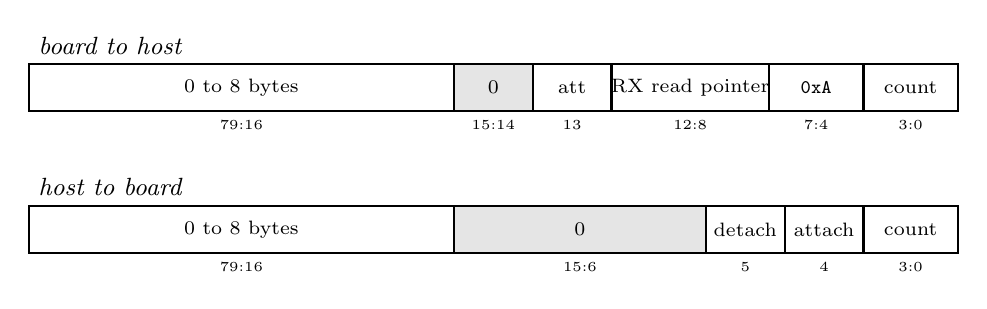
\begin{tikzpicture}[font=\scriptsize]
    \node[above right, font=\small\itshape] at (0,0.6) {board to host};
    \foreach \l/\r/\t/\b/\f in {0/5.4/{0 to 8 bytes}/{79:16}/white, 5.4/6.4/0/{15:14}/black!10, 6.4/7.4/att/13/white,
                                7.4/9.4/{RX read pointer}/{12:8}/white, 9.4/10.6/{\texttt{0xA}}/{7:4}/white, 10.6/11.8/count/{3:0}/white} {
      \draw[thick, fill=\f] (\l,0) rectangle (\r,0.6);
      \node at ({(\l+\r)/2},0.3) {\t};
      \node[below, font=\tiny] at ({(\l+\r)/2},0) {\b};
    }
    \begin{scope}[yshift=-1.8cm]
      \node[above right, font=\small\itshape] at (0,0.6) {host to board};
      \foreach \l/\r/\t/\b/\f in {0/5.4/{0 to 8 bytes}/{79:16}/white, 5.4/8.6/0/{15:6}/black!10, 8.6/9.6/detach/5/white,
                                  9.6/10.6/attach/4/white, 10.6/11.8/count/{3:0}/white} {
        \draw[thick, fill=\f] (\l,0) rectangle (\r,0.6);
        \node at ({(\l+\r)/2},0.3) {\t};
        \node[below, font=\tiny] at ({(\l+\r)/2},0) {\b};
      }
    \end{scope}
  \end{tikzpicture}
  \caption{The console frames (not to scale). The numbers below each field are its bits. Byte $i$ is at bit $16 + 8i$.}
  \label{fig:conframe}
\end{figure}

The \emph{att} bit shows that a host is attached. If no scan occurs for 0.67 s, the board clears the bit. While no host is attached, the board discards console output. Thus Linux does not stop when the FIFO is full and no host reads it.
